\subsection{Word Salience}

\begin{frame}{Deep Learning Models of Word Salience}


 
\textbf{Goal:} Make lexical information more useful for DL models of 
sentence extractive summarization.\\
~\\
\textbf{Why?} 
\begin{itemize}
 \item Improve performance.
 \item Improve explanation. 
 \item Improve generalizability.
 \end{itemize}
 \end{frame}

\begin{frame}{Word Features}

    \begin{itemize}
        \item Feature Embeddings
        \begin{itemize}
        \item Shallow lexical semantics (Glove Embeddings)
        \item<2-> Syntax
            \begin{itemize}
        \item POS tag
        \item Dependency role
        \item Dependency depth (distance from root node)
    \end{itemize}~\\
        \item<3-> Word Type/Topic
            \begin{itemize}
        \item Named-Entity tag
        \item LDA Topic/Brown Cluster 
             \end{itemize}~\\
         \item<4-> Term Probability
         \item<4-> Topic Signature
              \begin{itemize}
                  \item Log Likelihood Ratio (LLR): Log ratio of a term's document probability to  background corpus probability.
                \item Separate embeddings for words with highest LLR, and/or
                 \item separate embeddings for different thresholds of LLR.
              \end{itemize}

        \end{itemize}
~\\
        \item<5-> Contextualized representation (Elmo Embeddings)
    \end{itemize}


\end{frame}

\begin{frame}{Proposed Model}
    \begin{center}
    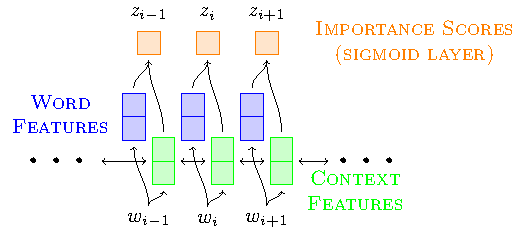
\includegraphics[scale=1.3]{3_deep_learning_models_of_salience/image_texs/wimp/wimp.pdf}

\end{center}




\end{frame}

\begin{frame}{Proposed Experiments}
\begin{itemize}
   \item<1-> Several ways to learn model:
           ~\\~\\
   \begin{itemize} 
     \item<2-> Learn as part of a sentence extractve summarization task.
     \begin{itemize}
        \item<3-> Margin based learning objective with greedy inference.
        \item<4-> Explore other combinatorial optimization algorithms, e.g. dynamic programming or ILP.
     \end{itemize}~\\~\\
     \item<5-> Directly supervision using reference summaries to classify words
     as in or out of the summary.
   \end{itemize}


\end{itemize}
\end{frame}

\begin{frame}{Proposed Experiments}
\begin{itemize}
   \item Learn word importance scores on large news datasets:
   \begin{itemize}
%     \item CNN/DailyMail 
%     \item NYT
     \item<2-> Newsroom (Grusky et al. 2018) 
         \begin{itemize}
             \item  1.3 million single document/summary pairs from news domain.
             \item Filterable subsections: extractive, abstractive, mixed.
             \end{itemize}~\\~\\
     \item<3-> XSUM (Narayan et al. 2018) 
         \begin{itemize}
             \item  200k  single document/summary pairs from news domain.
             \item More abstractive than previous datasets;
             \item requires 
                   combining information from multiple parts of the document.
           \end{itemize}
   \end{itemize}~\\
%   \item Many ways to construct a summary from $\omega$.
%    \item To start, greedy maximization of sum of importance scores, and
%    \item large margin learning frame work.

\end{itemize}
\end{frame}

%\begin{frame}{Large Margin Learning}
%
%    $\omega \triangleq $ Sentence $\times$ Term matrix of word salience 
%    weights, e.g. $\omega_{i,j}$ is the importance score of term $j$ 
%    in sentence $i$ \\
%
%    ~\\
%    $y \in \mathbb{Z}^n$ is an extractive reference summary of $n$ sentences.
%    ~\\
%    ~\\
%    $\eta \triangleq \sum_{j \in \{1, \ldots, |\mathcal{V}|\}} 
%        \max_{i \in y} \omega_{i,j},$ the score for the reference summary.
%    ~\\
%    ~\\
%    $\hat{y}, \hat{\eta}$ predicted summary indices and score.
%    ~\\
%    ~\\
%    $\mathcal{L}(y, \hat{y}) = \max\left(0, 1 + \hat{\eta} - \eta \right) $ 
%    ~\\
%    ~\\
%%    Auxiliary objective: $\mathcal{L}_{word}(z, \zeta) = -\sum_t \zeta_t \log z_t + (1 - \zeta_t) \log 1 - z_t  $ \\
%%   where $\zeta_t = 1$ if the $t$th input word occurs in the reference abstract
%%summary and 0 otherwise.
%
%\end{frame}

\begin{frame}{Other experiments/Plan B's}

    \begin{itemize}
%        \item We can supervise the individual importance scores using
%            the reference abstracts to get labels, i.e. $z_i \rightarrow 1$
%            if $w_i$ occurs in the reference summary.
%            ~\\~\\
%        \item More sophisticated inference, e.g. knapsack packing.~\\~\\
        %\item Matching performance of sentence extractive models ok if 
        %    word level scores gives additional explanability.
        \item Evaluate explainability: compare human judgements of word 
            importance to learned predictions
            ~\\~\\
        \item Genre Adaptation
            \begin{itemize}
                \item E.g. train adj/adv only news model and evaluate on Reddit.
            \end{itemize} ~\\
            \item Domain Adaptation to Multi-document Summarization
                \begin{itemize}
                    \item Encode documents individually
                    \item Aggregate importance scores using cross document attention
                \end{itemize}
    \end{itemize}
\end{frame}



%?\begin{frame}{Generalize to multi-document summarization}
%?\begin{enumerate}
%?\item For each document $d \in \{1, \ldots, D\}$ create word importance 
%?scores  $z_1^{(d)}, \ldots, z_{m_d}^{(d)}$.
%?\item Compute document set level attention matrix 
%?    $\Lambda \in \mathbb{R}^{M \times M}$ where $M = \sum_d^D m_d$ and 
%?\[ \Lambda_{i,j} = \sigma(h_i^Th_j / \tau + b)   \] and $h_i$ are outputs
%? of the contextual representation of the $i$-th word (e.g. ELMO embedding).
%?\item Compute aggregate importance scores $\bar{z_i} = \sum_{j=1}^M z_j \cdot \Lambda_{i, j}$ 
%?\item Create $\omega$ for all sentences in the document set using the aggregated scores  $\bar{z}_i$. 
%?\item Proceed as in the single-document summarization model.
%?\end{enumerate}
%?\end{frame}


\begin{frame}{Takeaways}

    \begin{itemize}
        \item Simple network architectures good enough. ~\\~\\
        \item Without care, document structure dominates learning. ~\\~\\
        \item To learn more from content, we propose to design better word 
            representations. ~\\~\\
    \end{itemize}

\end{frame}


%\begin{frame}{Supervise Attention for Abstractive Summarization}
%
%    \begin{itemize}
%        \item Normalized importance scores $z_i$ form a distribution over 
%            input tokens, like attention.
%        \item This could be used in a couple ways:
%            \begin{itemize}
%                \item Attention could be supervised to match the importance
%                    scores, i.e. supervising the content selection in the 
%                    decoder.
%                \item Directly masking the input to the decoder.
%            \end{itemize}
%    \end{itemize}
%
%\end{frame}
